\documentclass{article}

\usepackage{NeededPackages}


\begin{document}


\section{Introduction}
\begin{itemize}
    \item Each interrupt vector occupies two instruction Word(2x16bit) in Atmega328p.
    \item The complete placement of Reset and Interrupt Vectors in ATmega328P
    \begin{figure}[H]
        \begin{center}
            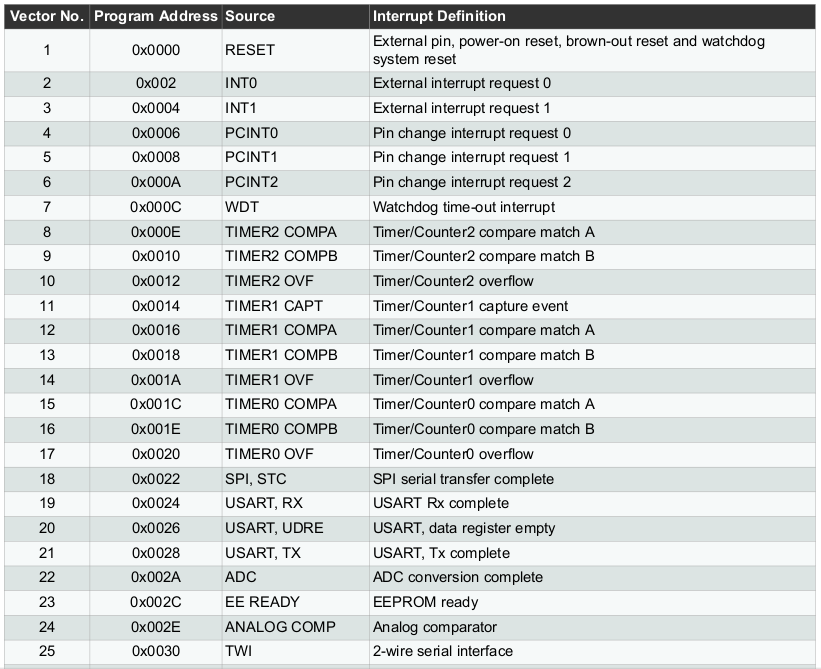
\includegraphics[height=.4\textheight]{resetAndInterruptVectors.png}
        \end{center}
    \end{figure}
    \item The location of reset vector is affected by \bitFormat{BOOTRST} fuse.
    \item The Interrupt vector start address is affected by \bitFormat{IVSEL} bit in \regFormat{MCUCR} register.
    \item The reset and interrupt Vector placement is shown below as
\end{itemize}
\begin{table}[H]
    \begin{minipage}{0.45\textwidth}
        \begin{center}
            \begin{tabular}{c|c}
                \bitFormat{BOOTRST} & \textbf{Reset Address}\\
                \hline
                0 & Boot reset address\\
                1 & 0x0000
            \end{tabular}
        \end{center}
    \end{minipage}
    \begin{minipage}{0.5\textwidth}
        \begin{center}
            \begin{tabular}{c|c}
                \bitFormat{IVSEL} & \textbf{Interrupt Vectors Start Address}\\
                \hline
                0 & 0x0002\\
                1 & Boot reset address + 0x0002
            \end{tabular}
        \end{center}
    \end{minipage}
\end{table}

\subsection{Register Description}
\subsubsection*{MCUCR – MCU Control Register}
\vspace*{0.5cm}
\begin{bytefield}[bitformatting={\large\bfseries},
    endianness=big,bitwidth=0.125\linewidth]{8}
    \bitheader[lsb=0]{0-7} \\
    \bitbox{1}{\small -}
    \bitbox{1}{\small BODS}
    \bitbox{1}{\small BODSE}
    \bitbox{1}{\small PUD}
    \bitbox{1}{\small -}
    \bitbox{1}{\small -}
    \bitbox{1}{\small IVSEL}
    \bitbox{1}{\small IVCE}\\
\end{bytefield}

\begin{itemize}
    \item When \bitFormat{IVSEL} bit is cleared, the interrupt vectors are placed at the start of the flash memory - the application section.
        \begin{itemize}
            \item When the \bitFormat{BLB12} is programmed, interrupts are disabled while executing from boot loader section.
        \end{itemize}
    \item When \bitFormat{IVSEL} bit is set, the interrupt vectors are moved to the beginning of the boot loader section of the flash. 
        \begin{itemize}
            \item When the \bitFormat{BLB02} is programmed, interrupts are disabled while executing from application section.
        \end{itemize}
    \item The actual address of the start of the boot flash section is determined by the \bitFormat{BOOTSZ} fuses.
    \item Writing \bitFormat{IVSEL} bit is done by
    \begin{enumerate}[label=(\alph*)]
        \item Write interrupt vector change enable \bitFormat{IVCE} bit to one.
        \item Write desired value to \bitFormat{IVSEL} while Writing zeros to \bitFormat{IVCE}.
    \end{enumerate}
    \item \bitFormat{IVCE} is cleared by hardware.
\end{itemize}

\section{External Interrupts}
\begin{itemize}
    \item Triggered by \pinFormat{INT0}, \pinFormat{INT1} and \pinFormat{PCING[23:0]} pins.
    \item Pin changed interrupt \emph{PCI2} will be triggered if any \pinFormat{PCINT[23:16]} toggles based on the \regFormat{PCMSK2} register.
    \item Pin changed interrupt \emph{PCI1} will be triggered if any \pinFormat{PCINT[14:8]} toggles based on the \regFormat{PCMSK1} register.
    \item Pin changed interrupt \emph{PCI0} will be triggered if any \pinFormat{PCINT[7:0]} toggles based on the \regFormat{PCMSK0} register.
    \item Due to asynchronous nature of Pin change interrupts, \pinFormat{PCINT[23:0]} can be used to wake up.
    \item The \pinFormat{INT0} and \pinFormat{INT1} can be triggered by falling, rising or low level choosen by \regFormat{EICRA} - External Interrupt Control Register.
    \item Due to asynchronous nature of External interrupts in low level interrupt, \pinFormat{INT0} and \pinFormat{INT1}  can be used to wake up.
 \end{itemize}

 \subsection{Register Description}
 \subsubsection*{EICRA - External Interrupt Control Register A}
 \vspace*{0.5cm}
\begin{bytefield}[bitformatting={\large\bfseries},
    endianness=big,bitwidth=0.125\linewidth]{8}
    \bitheader[lsb=0]{0-7} \\
    \bitbox{1}{\small -}
    \bitbox{1}{\small -}
    \bitbox{1}{\small -}
    \bitbox{1}{\small -}
    \bitbox{1}{\small ISC11}
    \bitbox{1}{\small ISC10}
    \bitbox{1}{\small ISC01}
    \bitbox{1}{\small ISC00}\\
\end{bytefield}

\begin{itemize}
    \item \bitFormat{ICS11:ICS10} - Interrupt Sense Control 1 Bit 1 and Bit 0
    \item \bitFormat{ICS01:ICS00} - Interrupt Sense Control 0 Bit 1 and Bit 0
\end{itemize}
\begin{table}[H]
    \begin{minipage}{0.45\textwidth}
        \begin{center}
            \begin{tabular}{c|p{5cm}}
                \bitFormat{ICS11:ICS10} & \textbf{Description}\\
                \hline
                00 & Low level of \bitFormat{INT1} generates interrupt\\
                01 & Any logic change on \bitFormat{INT1} generates interrupt\\
                10 & The falling edge of \bitFormat{INT1} generates an interrupt request.\\
                11 & The rising edge of \bitFormat{INT1} generates an interrupt request.\\
            \end{tabular}
        \end{center}
    \end{minipage}
    \begin{minipage}{0.45\textwidth}
        \begin{center}
            \begin{tabular}{c|p{5cm}}
                \bitFormat{ICS01:ICS00} & \textbf{Description}\\
                \hline
                00 & Low level of \bitFormat{INT0} generates interrupt\\
                01 & Any logic change on \bitFormat{INT0} generates interrupt\\
                10 & The falling edge of \bitFormat{INT0} generates an interrupt request.\\
                11 & The rising edge of \bitFormat{INT0} generates an interrupt request.\\
            \end{tabular}
        \end{center}
    \end{minipage}  
\end{table}

\subsubsection*{EIMSK – External Interrupt Mask Register}
\vspace*{0.5cm}
\begin{bytefield}[bitformatting={\large\bfseries},
    endianness=big,bitwidth=0.125\linewidth]{8}
    \bitheader[lsb=0]{0-7} \\
    \bitbox{1}{\small -}
    \bitbox{1}{\small -}
    \bitbox{1}{\small -}
    \bitbox{1}{\small -}
    \bitbox{1}{\small -}
    \bitbox{1}{\small -}
    \bitbox{1}{\small INT1}
    \bitbox{1}{\small INT0}\\
\end{bytefield}
\begin{itemize}
    \item Enable the corresponding External Interrupt Request Enable bits (\bitFormat{INT1} or \bitFormat{INT0}) and \bitFormat{I-biy} of status Register \regFormat{SREG} to enable the External interrupt.
\end{itemize}

\subsubsection*{EIFR – External Interrupt Flag Register}
\vspace*{0.5cm}
\begin{bytefield}[bitformatting={\large\bfseries},
    endianness=big,bitwidth=0.125\linewidth]{8}
    \bitheader[lsb=0]{0-7} \\
    \bitbox{1}{\small -}
    \bitbox{1}{\small -}
    \bitbox{1}{\small -}
    \bitbox{1}{\small -}
    \bitbox{1}{\small -}
    \bitbox{1}{\small -}
    \bitbox{1}{\small INTF1}
    \bitbox{1}{\small INTF0}\\
\end{bytefield}
\begin{itemize}
    \item When interrupt occurs on the External interrupt pins \pinFormat{INT0} and \pinFormat{INT1}, the corresponding External Interrupt Flag bits (\bitFormat{INTF1} or \bitFormat{INTF0}) are set.
    \item The Flag is cleared by by writing 1 to it in interrupt routine.
\end{itemize}

\subsubsection*{PCICR – Pin Change Interrupt Control Register}
\vspace*{0.5cm}
\begin{bytefield}[bitformatting={\large\bfseries},
    endianness=big,bitwidth=0.125\linewidth]{8}
    \bitheader[lsb=0]{0-7} \\
    \bitbox{1}{\small -}
    \bitbox{1}{\small -}
    \bitbox{1}{\small -}
    \bitbox{1}{\small -}
    \bitbox{1}{\small -}
    \bitbox{1}{\small PCIE2}
    \bitbox{1}{\small PCIE1}
    \bitbox{1}{\small PCIE0}\\
\end{bytefield}
\begin{itemize}
    \item Enable the corresponding Pin Change Interrupt Enable bits (\bitFormat{PCIE2} or \bitFormat{PCIE1} or \bitFormat{PCIE0}) and \bitFormat{I-bit} of status Register \regFormat{SREG} to enable the pin change interrupt.
    \item Setting 1 to \bitFormat{PCIE2} bit enabled interupt to occur  in \pinFormat{PCINT[23:16]} pins based on \regFormat{PCMSK2} register.
    \item Setting 1 to \bitFormat{PCIE1} bit enabled interupt to occur  in \pinFormat{PCINT[14:8]} pins based on \regFormat{PCMSK1} register.
    \item Setting 1 to \bitFormat{PCIE0} bit enabled interupt to occur  in \pinFormat{PCINT[7:0]} pins based on \regFormat{PCMSK0} register.
\end{itemize}

\subsubsection*{PCIFR – Pin Change Interrupt Flag Register}
\vspace*{0.5cm}
\begin{bytefield}[bitformatting={\large\bfseries},
    endianness=big,bitwidth=0.125\linewidth]{8}
    \bitheader[lsb=0]{0-7} \\
    \bitbox{1}{\small -}
    \bitbox{1}{\small -}
    \bitbox{1}{\small -}
    \bitbox{1}{\small -}
    \bitbox{1}{\small -}
    \bitbox{1}{\small PCIF2}
    \bitbox{1}{\small PCIF1}
    \bitbox{1}{\small PCIF0}\\
\end{bytefield}
\begin{itemize}
    \item When interrupt occurs on the Pin Change interrupt pins \pinFormat{PCINT[23:16]}, the \bitFormat{PCIF2} Pin Change Interrupt Flag 2 bits is set.
    \item When interrupt occurs on the Pin Change interrupt pins \pinFormat{PCINT[14:8]}, the \bitFormat{PCIF1} Pin Change Interrupt Flag 1 bits is set.
    \item When interrupt occurs on the Pin Change interrupt pins \pinFormat{PCINT[7:0]}, the \bitFormat{PCIF0} Pin Change Interrupt Flag 0 bits is set.
    \item The Flag is cleared by by writing 1 to it in interrupt routine.
\end{itemize}

\subsubsection*{PCMSK2 – Pin Change Mask Register 2}
\vspace*{0.5cm}
\begin{bytefield}[bitformatting={\large\bfseries},
    endianness=big,bitwidth=0.125\linewidth]{8}
    \bitheader[lsb=0]{0-7} \\
    \bitbox{1}{\small PCINT23}
    \bitbox{1}{\small PCINT22}
    \bitbox{1}{\small PCINT21}
    \bitbox{1}{\small PCINT20}
    \bitbox{1}{\small PCINT19}
    \bitbox{1}{\small PCINT18}
    \bitbox{1}{\small PCINT17}
    \bitbox{1}{\small PCINT16}\\
\end{bytefield}

\subsubsection*{PCMSK1 – Pin Chage Mask Register 1}
\vspace*{0.5cm}
\begin{bytefield}[bitformatting={\large\bfseries},
    endianness=big,bitwidth=0.125\linewidth]{8}
    \bitheader[lsb=0]{0-7} \\
    \bitbox{1}{\small -}
    \bitbox{1}{\small PCINT14}
    \bitbox{1}{\small PCINT13}
    \bitbox{1}{\small PCINT12}
    \bitbox{1}{\small PCINT11}
    \bitbox{1}{\small PCINT10}
    \bitbox{1}{\small PCINT9}
    \bitbox{1}{\small PCINT8}\\
\end{bytefield}

\subsubsection*{PCMSK0 – Pin Change Mask Register 0}
\vspace*{0.5cm}
\begin{bytefield}[bitformatting={\large\bfseries},
    endianness=big,bitwidth=0.125\linewidth]{8}
    \bitheader[lsb=0]{0-7} \\
    \bitbox{1}{\small PCINT7}
    \bitbox{1}{\small PCINT6}
    \bitbox{1}{\small PCINT5}
    \bitbox{1}{\small PCINT4}
    \bitbox{1}{\small PCINT3}
    \bitbox{1}{\small PCINT2}
    \bitbox{1}{\small PCINT1}
    \bitbox{1}{\small PCINT0}\\
\end{bytefield}
\begin{itemize}
    \item \regFormat{PCMSK2}, \regFormat{PCMSK1} and \regFormat{PCMSK0} are used to select which pin to be enabled for Pin Change Interrupt.
\end{itemize}

\section{Configuring External Interupt}
\begin{enumerate}[label=(\Roman*)]
    \item First, the \pinFormat{INT0} or \pinFormat{INT1} pins are configured as Input. (Optional)
    \item Next, the pull-up register may be enabled if needed.
    \item Next, the Interrupt Sense Control Bits are configured for level or edge triggered.
    \item Finally, the Interrupt are enabled.
    \item Also, Global interrupt is enabled.
    \item We define the ISR and check the Interrupt Flags if the interrupt occured.
    \item An example configuration can be seen below.
\end{enumerate}

\begin{minipage}{0.5\textwidth}
\begin{minted}[bgcolor=lightgray, breaklines]{c}
// making PD2 as input for INT0, though not neeced
DDRD &= ~(1<<2);
// enabling the internal pull-up register for PD2 for INT0
PORTD |= (1<<2);

// making EICRA's ISC01 and ISC00 as 10 for falling edge detection at INT0
EICRA |= (1<<ISC01);
EICRA &= ~(1<<ISC00);
// making EIMSK's INT0 as 1 to enable External Interrput Request for INT0
EIMSK |= (1<<INT0);

// Enabling global Interrupts
sei();	
\end{minted}
\end{minipage}
\begin{minipage}{0.45\textwidth}
\begin{minted}[bgcolor=lightgray, breaklines]{c}
ISR(INT0_vect)
{
    if((EIFR & (1<<INTF0)) != 0)	// INT0 interrupt as occured
    {		
        //toggle Led at pinc 0
        PINC |= (1<<0);
    }
}
\end{minted}
\end{minipage}


\section{Configuring Pin Change Interupt}
\begin{enumerate}[label=(\Roman*)]
    \item First, the \pinFormat{PCINT[23:0]} pins are configured as Input. (Optional)
    \item Next, the pull-up register may be enabled if needed.
    \item Next, which PCINT is selected.
    \item Finally, the Interrupt are enabled.
    \item Also, Global interrupt is enabled.
    \item We define the ISR and check the Interrupt Flags if the interrupt occured.
    \item An example configuration can be seen below.
\end{enumerate}

\begin{minipage}{0.5\textwidth}
\begin{minted}[bgcolor=lightgray, breaklines]{c}
// making PD4 as input for PCI20
DDRD &= ~(1<<4);
// enabling the internal pull-up register for PD4 for PCI20
PORTD |= (1<<4);

// Selecting the PCINT20 for PCI2 intterupt
PCMSK2 |= (1<<PCINT20);
// Enabling the PCI2 interupt
PCICR |= (1<<PCIE2);

// Enabling global Interrupts
sei();	
\end{minted}
\end{minipage}
\begin{minipage}{0.45\textwidth}
\begin{minted}[bgcolor=lightgray, breaklines]{c}
ISR(PCINT2_vect)
{
    if((PCIFR & (1<<PCIF2)) != 0)	// PCI2 interrupt as occured
    {		
        //toggle Led at pinc 0
        PINC |= (1<<0);

    }
}
\end{minted}
\end{minipage}



\end{document}

